\chapter{Vorgehensmodelle}

\section{Vorgehensmodelle in der Softwareentwicklung}

Vorgehensmodelle beantworten die wesentlichen Fragen der 
Organisation. Sie beschreibt das systematische, ingenieurmässig und quantifizierbare Vorgehen, um Aufgaben einer 
bestimmten Art wiederholbar zu lösen. Vorgehensmodelle werden hauptsächlich während Projektdurchführungsphase verwendet. Sie bilden eine Grundlage für die weitere Planung, die Projektüberwachung und die Projektsteuerung.

Sie bilden ein Instrument zur Integration von Methoden wie RE (Requirements Engineering) und Testen. Sie können anhand der W-Fragen strukturiert werden: Wer (--> Rollenmodell) erarbeitet Womit (--> Werkzeug \& Standards) Was (--> Artefakt-/Produktmodell) bis Wann (--> Ablaufmodell: Phase) und Wie (--> Aktivitätsmodell) geht er dabei vor? 

\section{Grundsätzliche Vorgehensmodelle}

Für Softwareprojekte stehen eine Reihe grundsätzlicher Vorgehensmodelle zur Verfügung. Die Modelle sollten auf das Projekt zugeschnitten werden (tailoring). Die Wahl für ein Modell erfolgt aufgrund des Projektcharakters.  \\
- Phasenmodell \\
- Spiralmodell \\
- Prototyping \\
- Agile Methoden \\

\subsection{Phasenmodell}
Das Phasenmodell ist ein klassischer Ansatz für die Organisation der Software- und Hardware-Entwicklung. Jede Phase erzeugt ein Ergebnis / Meilenstein, auf dem die nächste Phase aufbaut.

\subsection{Wasserfall-Modell}

\textbf{Philosophie:}  Aufteilung anhand Schwerpunkten der Entwicklungstätigkeiten 

\textbf{Phasen:} Analyse und Anforderung, Architekturentwurf, Implementation, Verifikation und Integration sowie Betrieb und Wartung

\textbf{Vorteile:} \\
- Einfache, klare Struktur \\
- Weitgehende Übereinstimmung des Artefakt- und Prozessmodells --> Vereinfacht scheinbar Planung, Organisation und Steuerung 

\textbf{Nachteile:} \\
- Planungs- und Entwicklungsfehler werden spät bemerkt  \\
- Risiken werden (zu) spät erkannt \\
- Umplanungen stehen im Gegensatz zur Philosophie und sind kostspielig \\
- Eine Rückkopplung aus der Implementationsphase findet sehr spät statt
- Enorme Erfahrung ist/wäre notwendig
\begin{figure}[ht]
	\centering
\adjustbox{width=12cm}{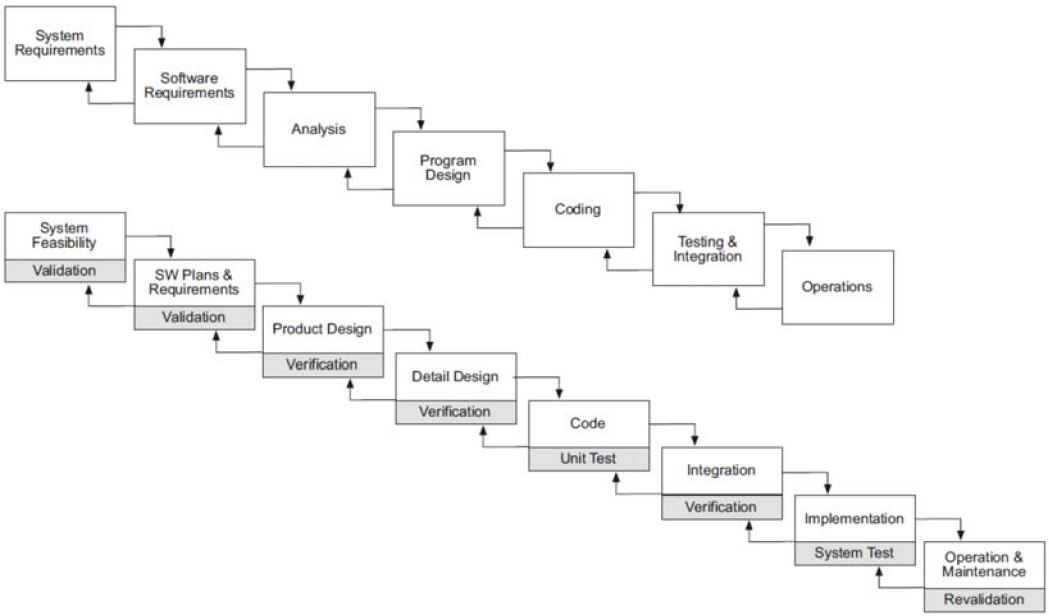
\includegraphics{Figures/wasserfall}}
\caption[]{Wasserfall - klassisch \& iterativ}
\end{figure}	
Iterativer Wasserfall: Kaskade; Erweiterung des Wasserfalls um Korrekturschleifen; In der Realität durchführbar (nicht wie der reine Wasserfall). Man kann immer nur eine Phase zurück

\subsection{V-Modell}
Grundidee: korrespondierende Tests \\
Erweiterung des Wasserfallmodells --> Ermahnt zum Testen
\begin{figure}[ht]
	\centering
	\adjustbox{width=8cm}{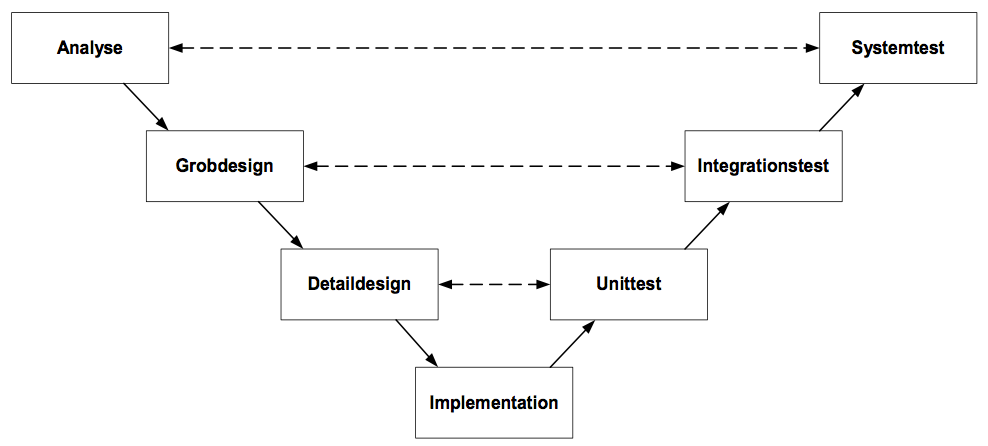
\includegraphics{Figures/v_modell}}
	\caption[]{V-Modell}
\end{figure}

\textbf{Vorteile:} \\
- Starke Einbindung der Test zu jeder Phase \\
- Klare, einfache Struktur \\
- Enorme Erfahrung aufgrund vorhandener Rückkopplung

\textbf{Nachteile:} \\
- kann zu inhaltlichen Problemen führen

\subsection{Spiralmodell}

Wiederholtes Durchlaufen der klassischen 
Entwicklungsphasen (Analyse, Evaluierung, Realisierung und Planung). Kontinuierliche Bereitstellung von 
Prototypen. Jede Iteration bringt den Prototypen näher 
an das endgültige Produkt. 

\textbf{Philosophie}
Erstellung von kontinuierlichen Prototypen und kontinuierliche Prüfung des System. Dies erlaubt kontinuierliche Lernkurven. Zudem werden die Ergebnisse der Zyklen wie Anforderungen oder Architekturen bei jeder Iteration verfeinert. Das weitere Vorgehen wird im 3. Schritt neu gewählt. Es ist kein Vorgehensmodell an sich, denn es sollte durch andere Vorgehensmodelle ausgestaltet werden. Im 4. Schritt kann allfällig eine Aufspaltung in Teilprojekte geschehen. 

\textbf{Inkrementelles Vorgehen} \\
Die Funktionalität wird schrittweise 
entwickelt bis das angestrebte System 
komplett ausgebaut ist. Iteratives Vorgehen ist zwingend nötig. 

\begin{figure}[ht]
	\centering
	\adjustbox{width=7cm}{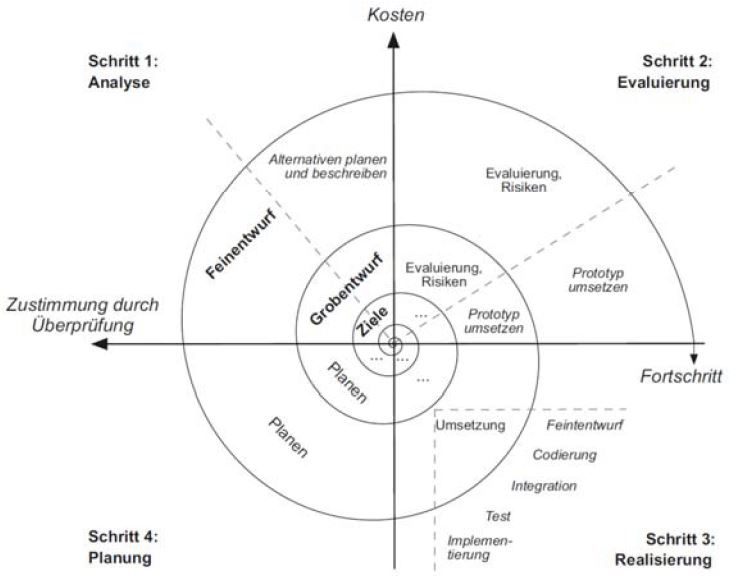
\includegraphics{Figures/spiralmodell}}
	\caption[]{Spiralmodell}
\end{figure}

\textbf{Vorteil:}
- Benötigt weniger Erfahrung als Wasserfallmodell, aufgrund der zugelassenen Lernkurven \\
- Risiken können frühzeitig erkannt werden

\subsection{Prototyping}
\begin{multicols}{2}
Prototyping beschreibt die frühe Realisierung ausgewählter oder kritischer Funktionen. Dabei geht es darum die Realisierung unter realitätsnahen Bedingungen zu zeigen. Es wird zur Prüfung der Machbarkeit, bei fehlender Erfahrung oder bei unklar definierten Anforderungen durchgeführt. \\
Anwendungen für Prototyping: bei User Interfaces, Smartphone Apps und Datenbanken
\columnbreak
Es wird zwischen einem horizontalem (Fokus auf eine Architekturebene) und vertikalen Prototyp (Fokus auf ein Funktionalität über alle Architekturebenen) unterschieden.
	\adjustbox{width=7.5cm}{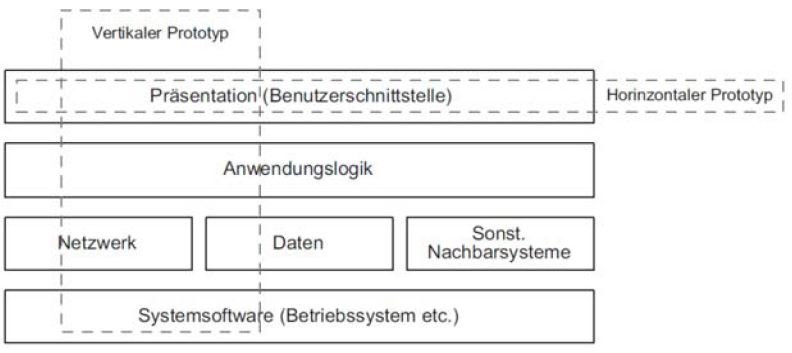
\includegraphics{Figures/formenvonprototyping}}

\end{multicols}

\subsection{Agile Methoden}
-  Gegensatz zu "schwergewichtigen" 
	Vorgehensweisen mit hohem Regelungs- und Organisationaufwand --> hohe Flexibilität, leichtgewichtiger Ansatz \\
- Agile = flink, beweglich / "Codezentriertes Vorgehen" \\

\textbf{Agiles Manifest (2001)}
- Individuen und Interaktionen mehr als 
Prozesse und Werkzeuge \\
- Funktionierende Software mehr als 
umfassende Dokumentation \\
- Zusammenarbeit mit dem Kunden mehr als 
Vertragsverhandlung \\
- Reagieren auf Veränderung mehr als das 
Befolgen eines Plans

Prominente Agile Methoden umfassen Refactoring, Pair Programming, Test-driven Development, Continuous Integration, Planning Game / Poker

\textbf{Vorteil:} \\
- Vorgehen kann für einen Hardware unabhängigen Teil der Software sinnvoll sein --> Stichwort "Hybrides Modell" \\
- Wertvolle Methoden: Refactoring / Test-Driven Development --> v.a. für erfahrene Programmierer

\textbf{Nachteil:} \\
Schwierig bei Hardwareentwicklung, da Anforderungen nicht zwingend von Anfang definiert

\section{Konkrete Vorgehensmodelle}
Die hier vorgestellten Modelle basieren auf den bereits gezeigten grundlegenden Philosophien. Die dabei grob beschriebenen Vorgehensmodelle eignen sich nur bedingt für die unmittelbare 
Anwendung in Projekten.


\subsection{Scrum}

Bei Scrum organisiert sich das Team weitgehend selbst. Die Grundannahme ist, dass Projekte komplex sind und somit nicht von Anfang an detailliert planbar sind. Am Anfang wird ein grober Projektrahmen definiert, indem sich das Team selbstorganisierend bewegt.

\begin{figure}[ht]
	\centering
	\adjustbox{width=10cm}{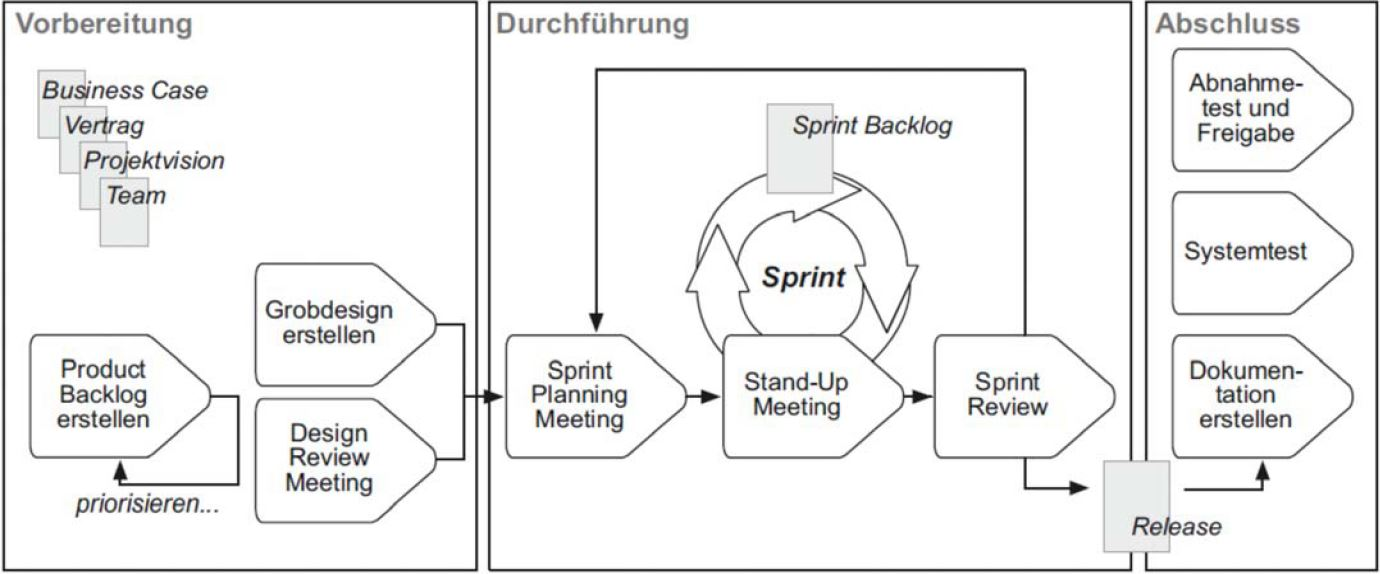
\includegraphics{Figures/scrum}}
	\caption[]{Scrum Prozess}
\end{figure} 
Basis: Sprints von 15-30 Tagen

\subsection{Rational Unified Process (RUP)}
RUP wurde von IBM Rational erfunden und wird kommerziell vertrieben. Es handelt sich um ein objektorientiertes, aktivitätsgetriebenes Vorgehensmodell, welches stark auf UML ausgerichtet ist. 
Grundprinzipien: \\
- Anwendungsfallgetrieben \\
-Die Architektur steht im Zentrum der Planung \\
- Das Vorgehen zur Entwicklung ist 
inkrementell/iterativ \\

\begin{figure}[ht]
	\centering
	\adjustbox{width=9cm}{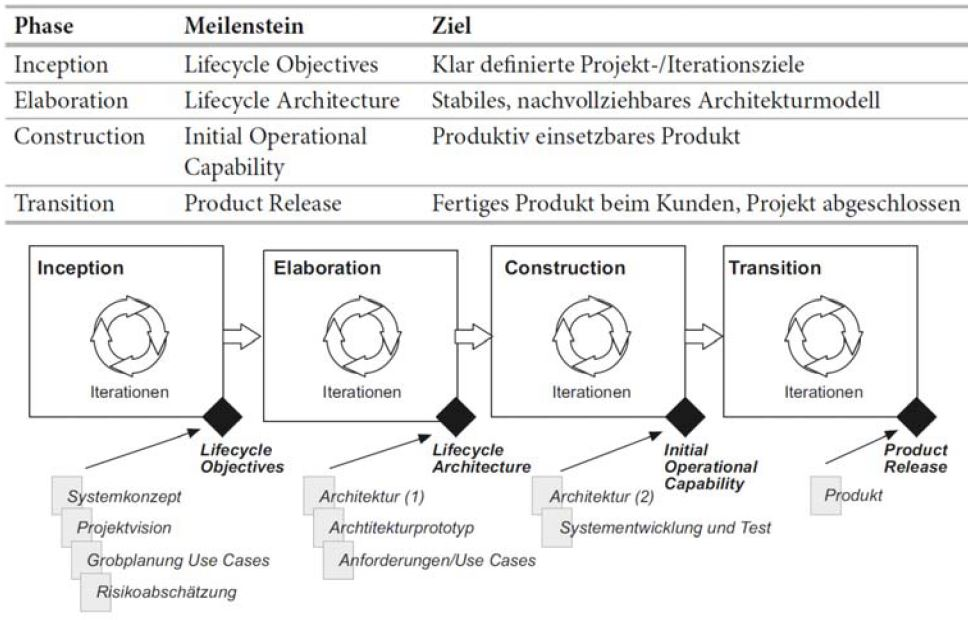
\includegraphics{Figures/RUP}}
\end{figure} 

\subsection{Diskussion der Vorgehensmodelle}
\begin{figure}[ht]
	\centering
	\adjustbox{width=15cm}{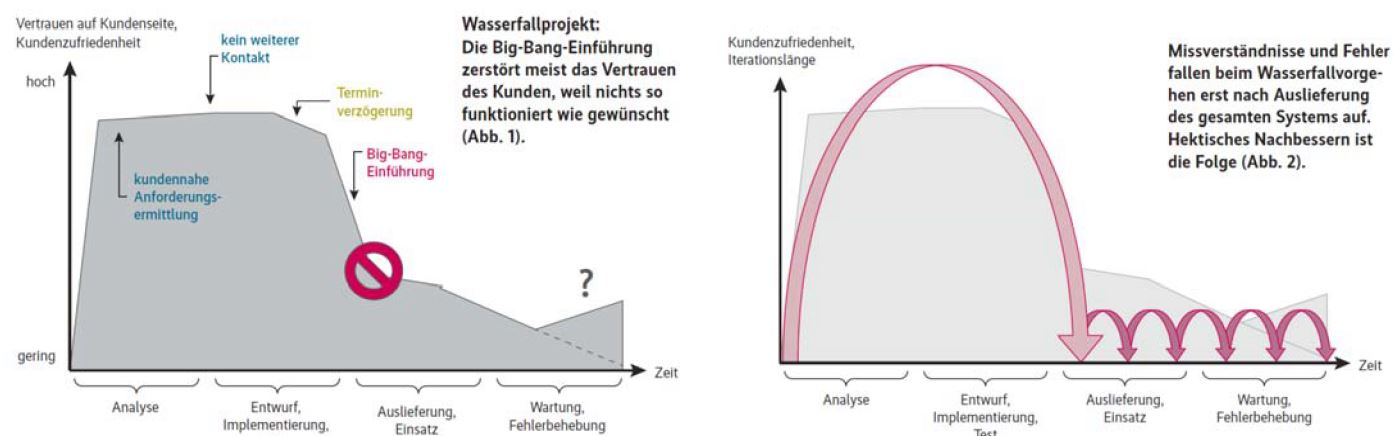
\includegraphics{Figures/diskussionvorgehensmodell}}
	\caption[]{Diskussion der Vorgehensmodelle}
\end{figure} 

\subsubsection{Brook'sche Regel}
\textit{Adding manpower to a late project makes it later} \\
Problem: Kommunikationsaufwand wird massiv erhöht.


